\begin{tikzpicture}
    \node at (0,0) {
    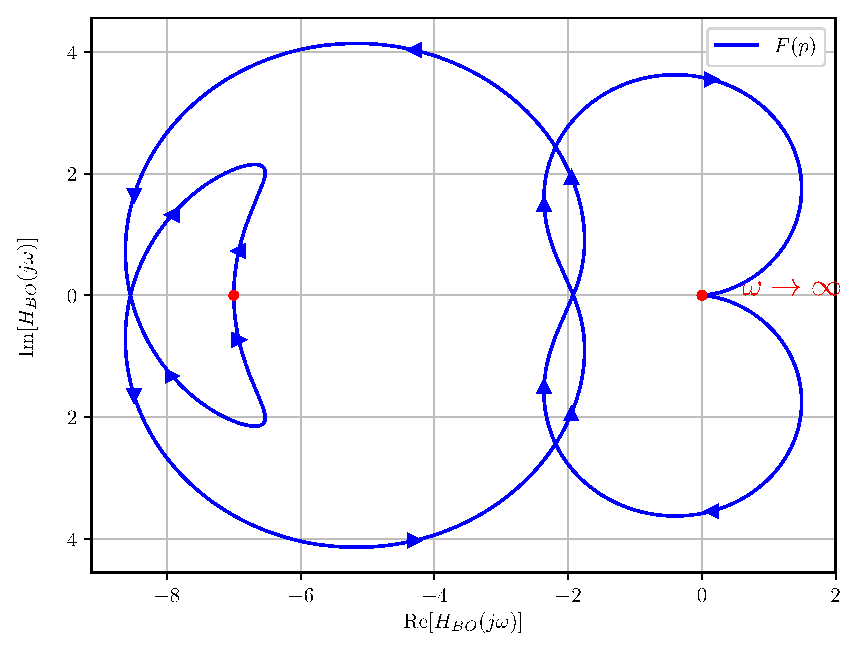
\includegraphics
    [width=0.8\textwidth]
    {fig/chap_stab/exercice_nyquist_chap_stab_ex1_enonce.eps}};
    \pgfmathsetmacro{\xu}{-4.28}
    \pgfmathsetmacro{\yu}{0.43}
    \draw[red,fill=red] (\xu,\yu) circle (1.62pt) node[above left] 
    {\textbf{I$_1$}};
    \pgfmathsetmacro{\xd}{-2.8}
    \pgfmathsetmacro{\yd}{0.43}
    \draw[red,fill=red] (\xd,\yd) circle (1.62pt) node[above right] 
    {\textbf{I$_2$}};
\end{tikzpicture}
